\documentclass{ctuthesis}
\usepackage{listings}
\usepackage{color}
\usepackage{multicol}
\usepackage{amsmath}
\usepackage{smartdiagram}
\usepackage{tikz}
\usetikzlibrary{shapes, angles, calc, quotes,arrows,automata, positioning}


\definecolor{dkgreen}{rgb}{0,0.6,0}
\definecolor{gray}{rgb}{0.5,0.5,0.5}
\definecolor{mauve}{rgb}{0.58,0,0.82}
\definecolor{variablesColor}{rgb}{0.66,0.46,0}
\DeclareMathOperator*{\argmax}{arg\,max}

\newcommand{\sign}[1]{%      
  \begin{tabular}[t]{@{}l@{}}
  \makebox[1.5in]{\dotfill}\\
  \strut#1\strut
  \end{tabular}%
}

\lstdefinelanguage{JASL}{
	keywordstyle=\color{blue},
    sensitive=true, % keywords are case-sensitive
    morecomment=[l]{\%}, % l is for line comment
    morestring=[b]", % defines that strings are enclosed in double quotes
    moredelim=[is][\color{variablesColor}]{|}{|},
    basicstyle=\ttfamily,
    emph={eps, circo, neato, dot, twopi},
    emphstyle=\color{mauve},
    numbers=left,
    morekeywords={Automaton, reduce, toCSV, fromCSV, toDot, toSimpleDot, accepts, toRegex, fromRegex, getExample, equals, help, helpLong, getTikzIncludes, union, intersection, kleene, concatenation, complement, execute, renameState, renameTerminal, toTikz, save},
} 

\lstdefinelanguage{JASL_snippet}{
	keywordstyle=\color{blue},
	sensitive=true,
	morecomment=[l]{\%}, % l is for line comment
    morestring=[b]", % defines that strings are enclosed in double quotes
    moredelim=[is][\color{variablesColor}]{|}{|},
    basicstyle=\ttfamily,
    emph={eps, circo, neato, dot, twopi},
    emphstyle=\color{mauve},
    numbers=none,
    morekeywords={Automaton, reduce, toCSV, fromCSV, toDot, toSimpleDot, accepts, toRegex, fromRegex, getExample, equals, help, helpLong, getTikzIncludes, union, intersection, kleene, concatenation, complement, execute, renameState, renameTerminal, toTikz, save},
}

\lstset{frame=tb,
  language=JASL,
  aboveskip=3mm,
  belowskip=3mm,
  showstringspaces=false,
  columns=flexible,
  basicstyle={\small\ttfamily},
  numberstyle=\small,
  keywordstyle=\color{blue},
  commentstyle=\color{dkgreen},
  stringstyle=\color{mauve},
  breaklines=true,
  breakatwhitespace=true,
  tabsize=3
}

\ctusetup{
xdoctype = B,
xfaculty = F3,
mainlanguage = english,
titlelanguage = english,
title-english = {Finite Automata Drawing Platform},
title-czech = {Platforma pro kreslení diagramů konečných automatů},
department-english = {Department of Cybernetics},
department-czech = {Katedra kybernetiky},
author = {Tomáš Hořovský},
supervisor = {RNDr. Marko Genyk-Berezovskyj},
supervisor-address = {Praha, Na Zderaze 269/4, room: G-9},
keywords-english = {Java, Automata theory, Regular automaton, Regular expression, Graphviz, JAutomata},
keywords-czech = { Java, Teorie automatů, Regulární automat, Regulární výraz, Graphviz, JAutomata},
month = 1,
year = 2019,
specification-file = zadani.pdf,
}

\ctuprocess

\begin{abstract-english}
The goal of this project was to develop new scripting language for describing automata and operations with them, implement interactive shell interface for executing the commands and finalize the \textbf{jautomata} library for operations on automata. The interpreter operates the \textbf{jautomata} library and implements export of automata to various output formats including \TeX code to display the automaton. 
\end{abstract-english}

\begin{abstract-czech}
Cílem tohoto projektu bylo dokončení knihovny \textbf{JAutomata} pro operace s automaty, vývoj nového skriptovacího jazyka \textbf{JASL}, který popisuje automaty a operace s těmito automaty a implementace interaktivního konzolového prostředí pro spouštění příkazů tohoto jazyka, které používá knihovnu JAutomata. Skriptovací jazyk JASL měl umožňovat export automatů v různých formátech, včetně kódu pro jazyk \TeX, pro kreslení jejich stavových diagramů.
\end{abstract-czech}


\begin{thanks}
I want to thank RNDr. Marko Genyk-Berezovskyj and prof. RNDr. Marie Demlová, CSc. for their help. I am also thankful to my family for their endless support.
\end{thanks}

\begin{declaration}
Prohlašuji, že jsem předloženou práci vypracoval samostatně a že jsem uvedl
veškeré použité informační zdroje v souladu s Metodickým pokynem o
dodržování etických principů při přípravě vysokoškolských závěrečných prací. \\
V Praze dne 7.1.2019 \\\par
\sign{Tomáš Hořovský}
\end{declaration}

\setlength{\parskip}{1em}

\begin{document}

\maketitle

\chapter{Introduction and motivation}
Java Automata Syntax Language (abbreviated to JASL) is a scripting language that I developed as a part of this project. It allows the user to define and work with acceptor finite state machines. I implemented an interpreter for this language that functions as a live console environment. One of the main features of JASL is the ability to export state machines to diagrams in a format native to \TeX.

Both jautomata library and JASL interpreter are written in pure object-oriented Java. The program should be able to run on Linux and Windows operating systems, but the primary support is for Linux.

This project started as a passion of mine for automata. I implemented a library in c++ that could do reduction of automata. I kept adding new functionality until the original automata-cpp library was so messy I could not orient in the code very well. After some time of struggling with the code, I needed to choose the assignment for my software project and my bachelor's thesis. It was only natural that I would finish and rewrite the whole library properly. \textbf{JAutomata} library was the result. I wrote most of the \textbf{JAutomata} library in my software project. I finished the library and I started working on \textbf{JASL} and the interpreter in my bachelor's thesis . 

\subsection{Motivation}

When I wrote my own material for Automata and Grammars in \LaTeX, I stumbled upon the problem of visualizing automata in the document. I wanted a fast and reliable way to draw automaton diagrams in code, not having to include image files to the compilation folder. I searched for a suitable way to do so and I found \textbf{TikZ}. TikZ is a powerful image drawing library that has many features. I tried drawing automaton directly with TikZ, but the code was unnecessarily long and tedious to write. After a couple of diagrams I started looking for another option. Then I found a library for TikZ called \textbf{automata}. It was just what I was looking for. It could draw nodes and edges nicely while keeping the code simple and clear. 

Next problem on the line was to draw these diagrams so that they are as simple as possible. Mostly eliminating crossing edges did the trick. However the more complex the diagram got, the harder it was to eliminate those by hand. I used \textit{Graphviz} to do the layout work for me. Then it was all about the process of converting Graphviz output to the TikZ code.

Automata have a few common operations associated with them. These include reduction, deciding whether a word is accepted by the automaton, constructing automaton that accepts language $L = L_1 \cup L_2$ or even automaton that accepts $L^*$. I decided to create a library that would implement all of these operations and more. There are libraries that can do these operations such as Algorithms~Library~Toolkit~\cite{alg_lib_toolkit}, but it is complicated to use, it is not public and it cannot output directly to \LaTeX code. 

The goal of this project is to write a program that would implement an intuitive command line interface for operating my JAutomata library that contains most of the commonly-used algorithms for working with automata. Also, it would allow the user to convert automata to various output formats including \LaTeX code.

The implemented solution uses various other programs and libraries to make the codebase smaller. It uses tools such as \textbf{Graphviz} or \textbf{graphviz-java} library. 

\chapter{Definitions and terminology}
In this section, I will define terminology used in this thesis to describe the relation of the application and language theory. Some of the definitions in sections \ref{sec:languages-def},\ref{sec:operations-languages-def},\ref{sec:automaton-def} and \ref{sec:regex-def} are translations of \cite{demlova}.
 
\section{Languages}
\label{sec:languages-def}
\begin{itemize}
	\item \textbf{Alphabet} is a finite non-empty set $\Sigma$. Elements of $\Sigma$ are called \textbf{terminals}.
	\item \textbf{Word} $w$ \textbf{over an alphabet} $\Sigma$ is a finite sequence of terminals: $w = a_1a_2\ldots a_m, a \in \Sigma, m \geq 0$.
	\item \textbf{Length of word} $w$, denoted by $|w|$, is the number of terminals in the word $w$.
	\item \textbf{Empty word} $\varepsilon$ is a word that has length $|\varepsilon| = 0$ (i.e. does not contain a terminal).
	\item \textbf{All words over an alphabet} $\Sigma$, denoted by $\Sigma^*$, is a set of all words that can be created using terminals from $\Sigma$ (including $\varepsilon$).
	\item For two words $w_1, w_2 \in \Sigma^*, w_1 = a_1a_2\ldots a_m, w_2 = b_1b_2\ldots b_n$ the result of the \textbf{concatenation} operation is: $w_1w_2 = a_1a_2\ldots a_mb_1b_2\ldots b_n$.
	\item \textbf{Language} $L$ over an alphabet $\Sigma$ is any arbitrary subset of $\Sigma^*$.
\end{itemize}

\section{Operations over languages}
\label{sec:operations-languages-def}
We will use the following operations over languages in this thesis:
\begin{itemize}
	\item \textbf{Concatenation of languages} $L_1 \subseteq \Sigma^*_1, L_2 \subseteq \Sigma^*_2$ is a set that is defined as follows:
	\begin{equation*}
		L_1L_2 = \{w_1w_2 \mid w_1 \in L_1, w_2 \in L_2\} \subseteq (\Sigma_1 \cup \Sigma_2)^*
	\end{equation*}
	
	\item \textbf{Union of languages} $L_1 \subseteq \Sigma^*_1, L_2 \subseteq \Sigma^*_2$ is a set that is defined as follows:
	\begin{equation*}
		L_1\cup L_2 = \{w \mid w \in (L_1 \cup L_2) \} \subseteq (\Sigma_1^* \cup \Sigma_2^*)
	\end{equation*}
	
	\item \textbf{Intersection of languages} $L_1 \subseteq \Sigma^*_1, L_2 \subseteq \Sigma^*_2$ is a set that is defined as follows:
	\begin{equation*}
		L_1 \cap L_2 = \{w \mid w \in L_1, w \in L_2 \} \subseteq (\Sigma^*_1 \cap \Sigma^*_2)
	\end{equation*}
	
	\item For any language $L$ we define $L^0 = \{\varepsilon\}, L^{i+1} = L^iL$ for $i \geq 0$. We define the result of \textbf{Kleene operation} as:
	\begin{equation*}
		L^* = \bigcup^{\infty}_{i=0} L^i
	\end{equation*}
	
	\item For any language $L$ over an alphabet $\Sigma$ we define its \textbf{complement} as: 
	\begin{equation*}
		\overline{L} = \{w | w \not \in L, w \in \Sigma^*\}
	\end{equation*}
\end{itemize}

\section{Automaton}
\label{sec:automaton-def}
The term automaton in language theory includes many types of automata, such as Moore automaton, Mealy automaton or others \cite{melichar}. However, JASL and JAutomata library implement only the following regular automata:
\subsection{Deterministic Finite Automaton (DFA)}
Deterministic Finite Automaton $M$ is defined as a tuple with five elements: $M = (Q, \Sigma, \delta, q_0, F)$, where:
\begin{itemize}
	\item $Q$ is a finite non-empty set of states.
	\item $\Sigma$ is a finite non-empty set of terminals
	\item $\delta$ is a transition function $\delta : Q \times \Sigma \rightarrow Q$
	\item $q_0$ is an initial state from the set $Q$
	\item $F$ is a subset of so-called accepting states, $F \subseteq Q$.
\end{itemize}

For the purpose of this thesis, we will interchangegably use the term \textbf{state} and \textbf{name of state} to call an element of $Q$ and we say that state name can be any string.

We define the \textbf{extended transition function} $\delta^* : Q \times \Sigma^* \rightarrow Q$ by induction as:  
\begin{align*}
	&1: \delta^*(q, \varepsilon) = q, &q \in Q \\
	&2: \delta^*(q, wa) = \delta(\delta^*(q, w), a), &a \in \Sigma, w \in \Sigma^*, q \in Q
\end{align*}

We say that automaton $M$ \textbf{accepts} word $w$ iff:
\begin{equation*}
	\delta^*(q_0, w) \in F
\end{equation*}


For an automaton $M$ over $\Sigma$, we define $L(M)$ (language accepted by $M$) as follows:
\begin{equation*}
	L(M) = \{w \mid \delta^*(q_0, w) \in F, w \in \Sigma^*\}
\end{equation*}

We say that states $p, q \in Q$ are \textbf{equivalent} iff:
\begin{equation*}
\forall w \in \Sigma^*, \delta^*(p, w) \in F \iff \delta^*(q, w) \in F
\end{equation*}

We say, that $M = (Q, \Sigma, \delta, q_0, F)$ is \textbf{reduced} if it does not have any unreachable states ($\forall q \in Q, \exists w \in \Sigma^*, \delta^*(q_0, w) = q$) and no two states of this automaton are equivalent.

We can informally describe the operation of an automaton as follows: \\
Suppose we have a word $w$ and an automaton $M$. We start in initial state of the automaton: $q_0$. We read the first terminal $a$ of the word and move to the state $q_1$ that we got as a result of $\delta(q_0, a)$. Now we have only $|w| - 1$ terminals left to read. We read the second terminal $b$. We move to the state $q_3$ that is the result of $\delta(q_1, b)$. We repeat this process, until we have no more terminals to read. Suppose we finished in state $q_7$. We say that word $w$ is accepted by automaton $M$ iff $q_7 \in F$.  

\subsection{Non-deterministic Finite Automaton (NFA)}
Non-deterministic Finite Automaton is a tuple: $M = (Q, \Sigma, \delta, I, F)$. Sets $Q, \Sigma, F$ have the same meaning as in DFA definition and: 
\begin{itemize}
	\item $I$ is a set of states that are considered initial: $I \subseteq Q$
	\item $\delta : Q \times X \rightarrow P(Q), P(Q)$ is a set of all subsets of states: $P(Q) = \{X \mid X \subseteq Q\}$
\end{itemize}

We define extended transition function for NFA as $\delta^* : Q \times \Sigma^* \rightarrow P(Q)$ by induction as:
\begin{align*}
	&1: \delta^*(q, \varepsilon) = \{q\}, &q \in Q \\
	&2: \delta^*(q, wa) = \bigcup\{\delta(p, a) \mid p \in \delta^*(q, w)\}, &a \in \Sigma, w \in \Sigma^*, q \in Q
\end{align*}

We say that NFA $M$ accepts word $w$ iff:
\begin{equation*}
	\exists q_0 \in I, \text{ such that } \delta^*(q_0, w) \cap F \ne \emptyset
\end{equation*}

\subsection{Non-deterministic Finite Automaton with epsilon transitions (ENFA)}
ENFA differs from NFA by introducing so-called $\varepsilon$-transitions. These allow the automaton to move between states without reading any terminal. Formally we change the transition function as follows:
\begin{equation*}
	\delta: Q \times (\Sigma \cup \{\varepsilon\}) \rightarrow P(Q)
\end{equation*}

To define extended transition function for ENFA, we need $\varepsilon$-closure. We can say that the epsilon closure of a set of states: $N$, is the set of all states that can be reached from states in $N$, using only epsilon transitions. 

We define $\varepsilon$-closure formally as:
\begin{enumerate}
	\item $\forall X \subseteq Q, X \subseteq \varepsilon$-closure$(X)$
	\item If $p \in \varepsilon$-closure$(X)$, then $\delta(p, \varepsilon) \subseteq \varepsilon$-closure$(X)$
\end{enumerate}

Now we can define extended transition function as:
\begin{align*}
	&1: \delta^*(q, \varepsilon) = \varepsilon\text{-closure}(q), &q \in Q \\
	&2: \delta^*(q, wa) = \cup\{\varepsilon\text{-closure}(\delta(p, a)) \mid p \in \delta^*(q, w)\}, &a \in \Sigma, w \in \Sigma^*
\end{align*}

We say that ENFA $M$ accepts word $w$ iff:
\begin{equation*}
	\exists q_0 \in I, \text{ such that } \delta^*(q_0, w) \cap F \ne \emptyset
\end{equation*}

\section{Regular expression}
\label{sec:regex-def}
A regular expression (regex) can describe any regular language (language accepted by some regular automaton). In this section, we will use bold font to denote regular expressions. In \cite{demlova} regular expressions are defined as follows:

Suppose we have an alphabet $\Sigma$. The set of all regular expressions over $\Sigma$ is defined as:
\begin{itemize}
	\item $\mathbf{\emptyset}$ is a regular expression
	\item $\mathbf{\varepsilon}$ is a regular expression
	\item \textbf{a} is a regular expression for every terminal $a \in \Sigma$
	\item If $\mathbf{r_1}, \mathbf{r_2}$ are regular expressions, then $\mathbf{r_1+r_2}, \mathbf{r_1r_2}$ and $\mathbf{r_1^*}$ are regular expressions
\end{itemize}

Every regular expression over an alphabet $\Sigma$ represents a language over an alphabet $\Sigma$ as follows: 
\begin{itemize}
	\item Regular expression $\boldsymbol{\emptyset}$ represents language $\emptyset$.
	\item Regular expression $\boldsymbol{\varepsilon}$ represents language $\{\varepsilon\}$.
	\item If $a \in \Sigma$ then regular expression: $\mathbf{a}$ represents language $\{a\}$.
	\item If regular expression $\mathbf{r_1}$ represents language $L_1$ and regular expression $\mathbf{r_2}$ represents language $L_2$, then regular expression $\mathbf{r_1 + r_2}$ represents language $L_1 \cup L_2$, and regular expression $\mathbf{r_1r_2}$ represents language $L_1L_2$.
	\item If regular expression $\mathbf{r}$ represents language $L$, then regular expression $\mathbf{r^*}$ represents language $L^*$.
\end{itemize}

Brackets in regular expressions define the order of operations. Regular expression $\mathbf{r}$ describes the same language as regular expression $\mathbf{(r)}$. 

\section{Notation of automata}
\subsection{Table}
\label{table}
In this thesis, automata are often described by their transition tables. Transition table has full information contained in the tuple $(Q, \Sigma, \delta, I, F)$. We construct this table from the tuple as follows:

The table has $k+2, k = |\Sigma|$ columns and $n+1, n = |Q|$ rows. In the first row of the table, there are two empty cells followed by all unique elements of $\Sigma$. The next $n$ rows are each for one state $q \in Q$. In the first column is $IO(q)$, which holds information about relation of $q$ to $I$ and $F$:

\begin{equation*}
	IO(q) = 
	\begin{cases}
		\rightarrow, & \quad \text{if } q \in I \text{ and } q \not \in F \\
		\leftarrow, & \quad \text{if } q \not \in I \text{ and } q \in F \\
		\leftrightarrow, & \quad \text{if } q \in I \text{ and } q \in F \\
		\text{empty}, & \quad \text{otherwise.}  
	\end{cases}
\end{equation*}

%\begin{itemize}
%	\item If $q \in I$ and $q \not \in F$ there is the symbol $\rightarrow$.
%	\item If $q \in F$ and $q \not \in I$ there is the symbol $\leftarrow$.
%	\item If $q \in F$ and $q \in I$ there is the symbol $\leftrightarrow$.
%	\item If $q \not \in F$ and $q \not \in I$, the cell is empty.
%\end{itemize}

In the second column is the name of state $q$. The remaining cells describe the function $\delta$. For every column header $t \in \Sigma$ and state $q$ the cell contains the set $\delta(q, t)$. We will omit curly brackets of the sets to clean up the notation. 

The table that is the result of this process describes fully all of the elements of the tuple and can be easily reconstructed into the tuple.

\paragraph{Example}
Suppose we have a non-deterministic finite automaton $M = (\{q_0, q_1, q_2, q_3\}, \{0,1\}, \delta, \{q_0, q_1\}, \{q_0, q_3\})$, where $\delta$ is defined as:
\begin{align*}
	&\delta(q_0, 0) = \{q_1\}, &\delta(q_0, 1) = \emptyset, \\
	&\delta(q_1, 0) = \{q_2, q_3\}, &\delta(q_1, 1) = \{q_0\}, \\
	&\delta(q_2, 0) = \{q_1\}, &\delta(q_2, 1) = \emptyset, \\
	&\delta(q_3, 0) = \emptyset, &\delta(q_3, 1) = \emptyset. 
\end{align*}

The resulting transition table is on figure~\ref{fig:trans-table}:

\begin{figure}[H]
\begin{ctucolortab}
\begin{tabular}{cc|cc}
	&&$0$ & $1$ \\\hline
	$\leftrightarrow$ & $q_0$ & $q_1$ & $\emptyset$ \\
	$\rightarrow$ & $q_1$ & $q_2,q_3$ & $q_0$ \\
	& $q_2$ & $q_1$ & $\emptyset$ \\
	$\leftarrow$ & $q_3$ & $\emptyset$ & $\emptyset$
\end{tabular}
\end{ctucolortab}
\caption{Transition table of automaton $M$}
\label{fig:trans-table}
\end{figure}

\section{State diagram}
One of the many use-cases for JASL is to output \TeX code to draw state diagrams of automata. A state diagram is a visual representation of an automaton. It provides a complete description of the automaton it is visualizing. A state diagram is a directed graph. Ullman and Hopcroft define it in 
\cite[Example 3.1, p.27]{hopcroft} as follows:
\begin{quote}
	"The state diagram consists of a node for every state and a directed line from state $q$ to state $p$ with label $a$ (in $\Sigma$) if the finite automaton, in state $q$, scanning the input symbol $a$, would go to state $p$. Final states, i.e., states in $F$, are indicated by a double circle."
\end{quote}

Ullman and Hopcroft use an arrow with label \textit{start}, to mark the initial state. We will omit the label, cleaning up the visuals of state diagrams. If we have multiple oriented edges from state $q_0$ to state $q_1$, we use only one edge labeled by the comma-delimited labels of all edges from $q_0$ to $q_1$. We will use dotted edges to emphasize $\varepsilon$ transitions in the diagram.

\paragraph{Example} A state diagram of the automaton $M$ from Example in section~\ref{table}, is in figure~\ref{fig:example-diagram}

\begin{figure}[H]
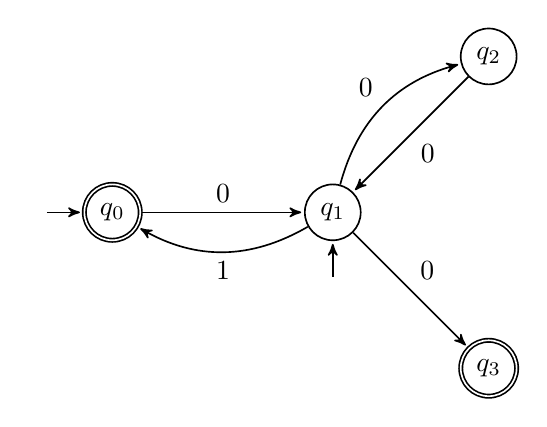
\begin{tikzpicture}[->,>=stealth',shorten >=1pt,auto,node distance=2.8cm,semithick,initial text=$ 	$]
	\tikzset{every state/.style={minimum size=0pt}}
	\node[state, initial, initial where=left, accepting] (0)  {$q_0$};
	\node[state, initial, initial where=below] (1) [right of=0] {$q_1$};
	\node[state] (2)[above right of=1]  {$q_2$};
	\node[state, accepting] (3) [below right of=1] {$q_3$};
	\path
		(0)

			edge node {$0$} (1)
		(1)

			edge [bend left] node {$1$} (0)
			edge [bend left] node {$0$} (2)
			edge  node {$0$} (3)
		(2)

			edge node {$0$} (1);
\end{tikzpicture}
\caption{State diagram of automaton $M$}
\label{fig:example-diagram}
\end{figure}

\chapter{User manual}
\section{Installation}
There are two ways of installing this program. You can either download precompiled .jar file or compile it on your own. If you just want to use the precompiled jar, skip right to the running section~\ref{sec:execution}

\subsection{Compiling JAR yourself}
\label{compile}
If you want to compile it yourself, you have to get the source code of the project from the official github repository~\cite{repo}. After that, you can install it using \cite{maven} and \cite{jdk}. 

Open a console in the root directory of the downloaded project and run these commands:
\begin{verbatim}
	mvn clean
	mvn install
\end{verbatim}

After running these commands, you can find the compiled .jar file in the target/ folder. Use the compiled .jar with dependencies (jautomata-1.1-jar-with-dependencies.jar).

\section{Execution}
\label{sec:execution}
The program can be executed from the console with this command :

\begin{verbatim}
	java -jar <path-to-jar> [-f <path-to-file>] 
\end{verbatim}

Square brackets are optional. If the switch -f is not specified, the program will enter interactive shell mode where you can type in your command and get an immediate response. The environment will store your variables in the interpreter memory and you can manipulate them as described in section~\ref{subsec:syntax}. However after terminating the shell environment (by using the \textbf{quit} command) all variables in the interpreter memory are lost. The same effect can be achieved even without closing the environment by using the \textbf{clear} command. 

If switch -f is specified, the program will look for its argument, which should be the path to an existing file. JASL will then execute commands from this file line by line. Note, that all variables are lost after terminating the program. 

You can execute JASL script files from the live interpreter environment, by using the execute function (full description in section~\ref{subsec:execute}). 

\section{Syntax of the language}
\label{subsec:syntax}
The \textbf{JASL} language allows you to define variables and call functions upon those variables. Commands are parsed line by line.

\paragraph{Grammar of the language} The following is an abstract grammar describing the JASL language. Terminals are shown in red color. Square brackets enclose optional parameters. Vertical bars separate alternatives. Starting non-terminal is linethe starting non-terminal.

\begin{figure}[H]
\begin{ctucolortab}
\begin{tabular}{rcl}
	line &$\rightarrow$& expression | assignment | comment | command | $\varepsilon$ \\
	variable &$\rightarrow$& \textcolor{red}{\$}\textbf{variableName}\\
	comment &$\rightarrow$& \textcolor{red}{\%}\textbf{any} \\
	expression &$\rightarrow$& \textbf{string} | list | functionCall | variable\textcolor{red}{.}memberFCall | variable \\
	list &$\rightarrow$& \textcolor{red}{\{}listItems\textcolor{red}{\}} | \textcolor{red}{\{}\textcolor{red}{\}} \\
	assignment &$\rightarrow$& variable \textcolor{red}{ = } expression \\
	listItems &$\rightarrow$& expression | expression\textcolor{red}{,} listItems \\
	functionCall &$\rightarrow$& \textbf{functionName}\textcolor{red}{(}[args]\textcolor{red}{)}[\textcolor{red}{.}memberFCall] \\
	args &$\rightarrow$& expression[\textcolor{red}{,} args] \\
	memberFCall &$\rightarrow$& \textbf{memberFName}\textcolor{red}{(}[args]\textcolor{red}{)}[\textcolor{red}{.}memberFCall] \\
	command &$\rightarrow$& \textcolor{red}{help} | \textcolor{red}{helpLong} | \textcolor{red}{clear} 
\end{tabular}
\end{ctucolortab}
\end{figure}

where non-terminals:
\begin{itemize}
	\item \textbf{any} can be any sequence of characters that does not contain linebreak
	\item \textbf{variableName} can be any non-empty sequence of characters that does not contain any whitespace characters or dots. 
	\item \textbf{functionName} is any function name from chapter \ref{sec:functions}
	\item \textbf{memberFName} is any function name from chapter \ref{subsec:member-functions}
	\item \textbf{string} is any sequence of characters that does not start with any function name, member function name or any of these symbols: \textcolor{red}{\textbf{\{ , \% \$}} and does not contain linebreak
\end{itemize}

\subsection{Syntax details}

\paragraph{Expressions}
Expression is a function call, member function call, string or list definition. Expressions are evaluated before assignments. This evaluation typically produces a new value that contains the result of the evaluation. If an expression is called by itself, the console prints the return value.

\paragraph{Object} 
An object is a piece of data. 

\paragraph{Variables}
Variables are used to store objects. Variable name can be any string that does not contain whitespace or a dot. To access a variable (create variable or use existing variable), use this syntax:
\begin{verbatim}
	$<variableName>
\end{verbatim}

\paragraph{Assignment}
\begin{verbatim}
	<variable> = <expression>
\end{verbatim} 
Assignments save <expression> return value to an <variable>. This is done using '=' operator. If the variable does not exist, an assignment creates a new variable.

\paragraph{Functions}
Function calls consist of the name of the function followed by comma-separated arguments enclosed in a pair of parentheses. 
\begin{verbatim}
	<functionName>(<arguments>)
\end{verbatim}

\paragraph{Comments}
You can add comments to your JASL code by the means of line comments. This means that only a whole line can be a comment. Commenting at the end of a non-comment line is not possible. Every comment starts with the \textbf{\%} sign as the first character. Everything that follows the percent sign will not be parsed and the whole line will be skipped. 
\begin{verbatim}
	%<commentString>
\end{verbatim}

\paragraph{Help}
Help for the JASL syntax can be displayed with command: \textbf{help} while command: \textbf{helpLong} prints longer, more detailed version with descriptions of functions. 

\subsection{Data types}
Variables can hold objects of types: string, list or automaton.
\paragraph{String} Used mainly to describe terminals, words or regular expressions. A string can be any sequence of characters that does not contain any linebreak and does not start with any function name, member function name or any of these symbols: \textbf{\{ , \% \$}.
\paragraph{List}
List in JASL is an ordered set of elements. Lists are enclosed in pairs of curly brackets. Elements are separated by commas. Elements can be any objects. Lists can be empty and they can be nested. They are used for defining automata. Some examples of lists are:

\begin{minipage}{\linewidth}
\begin{lstlisting}[language = JASL_snippet]
	{a, b, c}
	{}
	{a, {b, {}}, c}
\end{lstlisting}
\end{minipage}

\paragraph{Automaton}
This data type is explained in section \ref{subsec:automata-variables}

\subsection{Functions}
\label{sec:functions}
In this section, I will describe the functions that are implemented in JASL in more detail. The code examples use assignments to indicate return type.

\subsubsection{execute}
\label{subsec:execute}
\begin{lstlisting}[language = JASL_snippet]
	execute(|$path|)
\end{lstlisting}

Executes script on the specified path. The argument is a string (or a variable that contains a string) that contains absolute or relative path to a file in filesystem. Execute uses already defined variables for the execution, and updates/overwrites them. This effect is demonstrated in section \ref{ex:exec-overwrite}.

A JASL script is a file that contains one or several lines of JASL code. It is recommended to give JASL scripts the .jasl extension.

\subsubsection{fromCSV}
\begin{lstlisting}[language = JASL_snippet]
	|$M| = fromCSV(|$path|)
\end{lstlisting}

Returns new Automaton object, loaded from a comma-separated csv file specified in the single argument of this function. The argument is a string (or a variable that contains a string) that contains absolute or relative path to a file in filesystem. The CSV file should contain the automaton table as described in section \ref{table}.

\subsubsection{getExample}
\begin{lstlisting}[language = JASL_snippet]
	|$automaton| = getExample()
\end{lstlisting}

Returns example automaton. The example automaton is described by this transition table:
\begin{table}[H]
\begin{ctucolortab}
\begin{tabular}{cc|c|c}
	 & & $a$ & $b$ \\\Midrule
	$\rightarrow$ & $0$ & $1$ & $2,3$ \\
	$\rightarrow$ & $1$ & & $1,4$ \\
	$\leftrightarrow$ & $2$ & & $0$ \\
	$\leftarrow$ & $3$ & $3$ & $3$ \\
	 & $4$ & $4$ & $2$ 
\end{tabular}
\end{ctucolortab}
\caption{Transition table of example automaton}
\label{fig:example_automaton_table}
\end{table}

And its state diagram:
\begin{figure}[H]
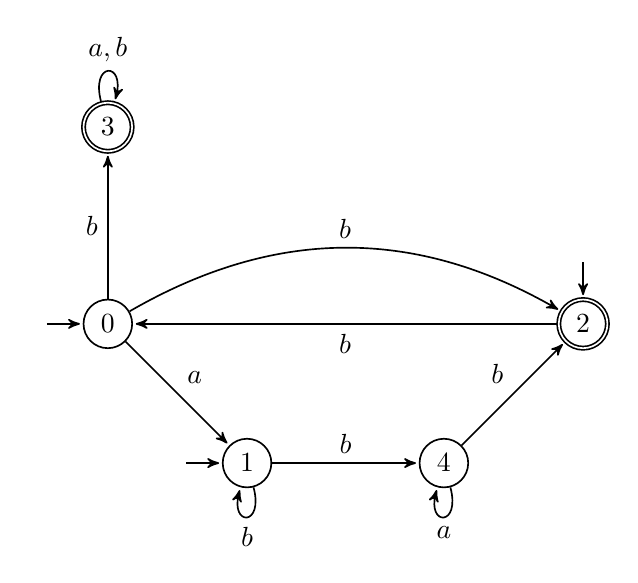
\begin{tikzpicture}[->,>=stealth',shorten >=1pt,auto,node distance=2.5cm,semithick,initial text=$ $]
	\tikzset{every state/.style={minimum size=0pt}}
	\node[state, initial, initial where=left] (0) {$0$};
	\node[state, initial, initial where=left] (1) [below right of=0] {$1$};
	\node[state] (4) [right of=1] {$4$};
	\node[state, initial, initial where=above, accepting] (2) [above right of=4] {$2$};
	\node[state, accepting] (3) [above of=0] {$3$};

	\path
		(0)

			edge node {$a$} (1)
			edge [bend left] node {$b$} (2)
			edge node {$b$} (3)
		(1)

			edge [loop below] node {$b$} (1)
			edge  node {$b$} (4)
		(2)

			edge node {$b$} (0)
		(3)

			edge [loop above] node {$a,b$} (3)
		(4)

			edge node {$b$} (2)
			edge [loop below] node {$a$} (4);
\end{tikzpicture}
\caption{State diagram of example automaton}
\label{fig:example_automaton_diagram}
\end{figure}

\subsubsection{fromRegex}
\label{fromRegex}
\begin{lstlisting}[language = JASL_snippet]
	|$automaton| = fromRegex(|$regex|)
\end{lstlisting}

Returns new Automaton object specified by regular expression passed in as an argument. The argument is a string or a variable that contains a string. The regular expression has to be in the format specified in chapter~\ref{sec:regex-def} or format described in section \ref{toRegex}.

There are limitations to this function. It works only with terminals that are a single character. Characters cannot be escaped, so symbols '\textbf{(}', '\textbf{)}', \textbf{\{}, \textbf{\}}, '$\mathbf{\cdot}$' and '\textbf{*}' cannot be used as terminals. 

The JAutomata library uses a modified version of the algorithm from \cite[p.86 algorithm 2.107]{melichar}, to create automata from regular expressions.

\subsubsection{getTikzIncludes}
\label{subsec:getTikzIncludes}
\begin{lstlisting}[language = JASL_snippet]
	getTikzIncludes()
\end{lstlisting}

Returns the \TeX includes needed, in order to use TikZ and its libraries that are necessary for diagrams of automata to work.

This code is:
\begin{verbatim}
	\usepackage{tikz}
	\usetikzlibrary{shapes,angles,calc,quotes,arrows,automata,positioning}
\end{verbatim}

\subsection{Automata}
\label{subsec:automata-variables}
To define an automaton you need to use the Automaton function. This function accepts a single parameter: nested list $L = \{l_s, l_1, l_2, \ldots, l_n\}, n = |Q|$, where $Q$ is the set of states of the automaton we want to define.  Elements of list $L$ are:
\begin{itemize}
	\item disjoint list of all terminals in $\Sigma$.
	\item n lists where each list $l_i = \{\text{IO}, q_i, \delta(q_i, t_1), \delta(q_i, t_2), \ldots, \delta(q_i, t_k)\}, \forall q_i \in Q, k = |Q|$, where $IO$ is defined as: 
 	
	$IO = 
		\begin{cases}
			\text{<>,} &\quad\text{if }q_i \in F, Q_i \in I \\
			\text{<,} &\quad\text{if }q_i \in F\\
			\text{>,} &\quad\text{if }q_i \in I \\
			\text{empty string,} &\quad\text{otherwise}\\
		\end{cases}$
\end{itemize}

In other words, this parameter is the transition table of the automaton. Lists in the definition are the rows of transition table read from left to right, separated by commas.

Example of conversion:
\begin{table}[H]
\begin{ctucolortab}
\begin{tabular}{cc|cc}
	&	& $a$	& $b$ \\\Midrule
$\leftrightarrow$	& $0$	& $\emptyset$	& $2$ \\
$\rightarrow$	& $1$ & $0$ & $1,2$ \\
$\leftarrow$	& $2$ & $1,2,3$ & $1$ \\
				& $3$ & $3$	& $\emptyset$ 
\end{tabular}
\quad
$\rightarrow$
\begin{tabular}{|c|c|c|c|}
\hline
	&&$a$&$b$ \\
	$<>$ & $0$ & $\{\}$ & $2$ \\
	$>$ & $1$ & $0$ & $\{1,2\}$ \\
	$<$ & $2$ & $\{1,2,3\}$ & $1$ \\
		& $3$ & $3$ & $\{\}$\\
		\hline
\end{tabular}
\quad 
$\rightarrow$
\begin{tabular}{|l|}
\hline 
$\{a, b\}$ \\
$\{<>,0,\{\}, 2\}$ \\
$\{>,1,0,\{1,2\}\}$ \\
$\{<,2,\{1,2,3\},1\}$ \\
$\{3, 3, \{\}\}$ \\\hline
\end{tabular}
\end{ctucolortab}
\caption{Example of conversion of transition table to list}
\label{fig:example_conversion}
\end{table}

So the argument to construct this automaton is:
\begin{lstlisting}[language = JASL_snippet]
	{{a,b},{<>,0,{},2},{>,1,0,{1,2}},{<,2,{1,2,3},1},{3,3,{}}}
\end{lstlisting}

The automaton specified by the transition table is NFA automaton. It is created by using the Automaton constructor. The definition of the nested list can be split into multiple list variables for the sake of clarity. We can also omit empty lists from the end of each row. This is demonstrated on lines 5-8:

\begin{minipage}{\linewidth}
\begin{lstlisting}[language = JASL]
	|$alphabet| = {a, b}
	|$row0|  = {<>,0,{},2}
	|$row1|  = {>,1,0,{1,2}}
	|$row2|  = {<,2,{1,2,3},1}
	% The full definition of row 3:
	|$row3|  = {3,3,{}}
	% Shortened definition of row 3:
	|$row3| = {3,3}
	
	% Now we define the nested list:
	|$nestedList| = {|$alphabet|, |$row0|, |$row1|, |$row2|, |$row3|}
    
	% Finally, we can define an automaton:
	|$automaton| = Automaton(|$nestedList|)
\end{lstlisting}
\end{minipage}

\paragraph{Note about ENFA automata}
ENFA automata can have $\varepsilon$-transitions. These are defined using keyword eps as one of the terminals. That terminal then signifies an $\varepsilon$ transition. The alphabet of some ENFA automaton could be:
\begin{lstlisting}[language = JASL]
	|$alphabet| = {eps, a, b}
\end{lstlisting} 

\subsection{Member functions}
\label{subsec:member-functions}
Member function is a function called on an object saved in a variable. There member function for types string and automaton. These can be invoked as follows:

\begin{minipage}{\linewidth}
\begin{lstlisting}[language = JASL_snippet]
	|$variable|.functionName(<list of args>)
\end{lstlisting}
\end{minipage} 

Note that member function calls can be chained on one line:

\begin{minipage}{\linewidth}
\begin{lstlisting}[language = JASL]
	|$reduced| = |$automaton|.reduced()
	|$reduced|.toPNG(image.png)
	
	% Can be written as:
	|$automaton|.reduced().toPNG(image.png)
\end{lstlisting}
\end{minipage}

String objects have only the \textbf{save} member function:

\subsubsection{save}
\begin{lstlisting}[language = JASL_snippet]
	|$myString|.save(|$path|)
\end{lstlisting}

Saves string saved in the variable \$myString to file at \$path. If the file does not exist, it creates it. If the file already exists, it appends the string to the end of the file. The argument is a string (or a variable that contains a string), that specifies a file in filesystem.

What follows is a list of member functions for automata objects. The notation for examples is the same as in section~\ref{sec:functions}

\subsubsection{accepts}
\begin{lstlisting}[language = JASL_snippet]
	|$M|.accepts($w)
\end{lstlisting}

Returns \textit{true} if automaton $M$ (saved in variable \$M) accepts word passed in argument ($w \in L(M)$). It outputs \textit{false} otherwise. The argument of this function can be a string or a list of terminals. If the argument is of type string, it is parsed character by character into terminals. Note, that if you have an automaton that has any terminals with more than one character, you cannot use the variant with the argument of type string. In that case you need to use a list as an argument.

Note, that this function works even if $w \not \in \Sigma^*$, where $\Sigma$ is the alphabet of automaton $M$. In that case it returns \textit{false}.

\subsubsection{equals}
\begin{lstlisting}[language = JASL_snippet]
	|$M1|.equals(|$M2|)
\end{lstlisting}

Returns \textit{true} if $L(M_1) = L(M_2)$ (if $M_1$ is equivalent to $M_2$). It outputs \textit{false} otherwise. In other words this function checks, whether two automata accept the same language. 

\subsubsection{reduce}
\begin{lstlisting}[language = JASL_snippet]
	|$M2| = |$M|.reduce()
\end{lstlisting}

Returns new automaton $M_2$ that is the reduced version of automaton $M$. Note that this function creates a new automaton object, so the original automaton remains unchanged. 

If the automaton $M$ is an ENFA automaton or an NFA automaton, it is first converted to DFA automaton, before the reduction. All of the described operations are implemented using respective algorithms from \cite{demlova}.

\subsubsection{toCSV}
\begin{lstlisting}[language = JASL_snippet]
	|$M|.toCSV(|$path|)
\end{lstlisting}

Exports automaton $M$ to CSV format. It creates/overwrites csv file on the path specified by the argument. The argument is a string that contains absolute or relative path to a file in the filesystem. The created CSV file contains the transition table of the automaton $M$.

\subsubsection{toDot}
\label{subsec:toDot}
\begin{lstlisting}[language = JASL_snippet]
	|$M|.toDot(neato)
\end{lstlisting}

Outputs attributed dot code (described in chapter \ref{drawing-images}), that contains a description of the automaton state diagram image. It accepts one, optional argument. The argument is the layout (engine) that Graphviz will use to organize the graph. When no layout is specified, \textbf{dot} is used as a default. Possible layouts are \textbf{circo}, \textbf{neato}, \textbf{dot} and \textbf{twopi}. 

\subsubsection{toPNG}
\begin{lstlisting}[language = JASL_snippet]
	|$M|.toPNG(|$path|, circo)
\end{lstlisting}

Exports automaton $M$ to PNG format. It creates/overwrites png file on the path specified by the argument. The argument is a string that contains absolute or relative path to a file in the filesystem. The png contains an image of the state diagram of the automaton $M$. 

The second argument of toPNG is optional. It is the layout (engine) that Graphviz will use to organize the graph. When no layout is specified, \textbf{dot} is used as a default. Possible layouts are \textbf{circo}, \textbf{neato}, \textbf{dot} and \textbf{twopi}.

\subsubsection{toRegex}
\label{toRegex}
\begin{lstlisting}[language = JASL_snippet]
	|$M|.toRegex()
\end{lstlisting}

Outputs regular expression describing language $L = L(M)$. Because no regular expression simplifier is implemented, the output of this function can be quite complicated. Nevertheless, it describes the language $L$. The output has a slightly different format from the definition in section \ref{sec:regex-def}. In the output, concatenation of languages generated by regular expressions $\mathbf{r_1}, \mathbf{r_2}$ is denoted by $\mathbf{r_1}\cdot \mathbf{r_2}$, instead of $\mathbf{r_1r_2}$. This format is also accepted by the fromRegex function \ref{fromRegex}.

To convert automaton to regular expression the JAutomata library uses a modified algorithm described in \cite[p.98 algorithm 2.120]{melichar}.

\subsubsection{toSimpleDot}
\begin{lstlisting}[language = JASL_snippet]
	|$M|.toSimpleDot()
\end{lstlisting}

Outputs dot code, that contains a description of the automaton state-diagram image. As opposed to \hyperref[subsec:toDot]{toDot} function, the dot code is not attributed, so it does not contain positions of elements.

\subsubsection{toTexTable}
\begin{lstlisting}[language = JASL_snippet]
	|$M|.toTexTable()
\end{lstlisting}

Outputs string containing \TeX code to display the transition table of automaton $M$. 

\subsubsection{toTikz}
\label{to-tikz-conversion}
\begin{lstlisting}[language = JASL_snippet]
	|$M|.toTikz(dot)
\end{lstlisting}

Outputs TikZ code to display the state diagram of automaton $M$. It accepts one parameter, that is the layout (engine) Graphviz will use to organize the graph. When no layout is specified, \textbf{dot} is used as a default. Possible layouts are \textbf{circo}, \textbf{neato}, \textbf{dot} and \textbf{twopi}. It is recommended not to specify this argument (hence use \textbf{dot} as an engine), because it generally outputs the nicest results out of the options. Note that you need to add appropriate includes to your \TeX code. You can get these using the \hyperref[subsec:getTikzIncludes]{getTikzIncludes} function.

\subsubsection{complement}
\begin{lstlisting}[language = JASL_snippet]
	|$M2| = |$M1|.complement()
\end{lstlisting}

Returns automaton that accepts language, that is the complement to the language of the original automaton.
\begin{equation*}
	L(M_2) = \overline{L(M_1)}
\end{equation*}

\subsubsection{concatenation}
\begin{lstlisting}[language = JASL_snippet]
	|$M3| = |$M1|.concatenation(|$M2|)
\end{lstlisting}

Outputs new automaton $M_3$ that accepts the concatenation of languages accepted by automata $M_1, M_2$. It accepts one argument of type automaton.
\begin{equation*}
	L(M_3) = L(M_1)L(M_2)
\end{equation*}

\subsubsection{intersection}
\begin{lstlisting}[language = JASL_snippet]
	|$M3| = |$M1|.intersection(|$M2|)
\end{lstlisting}

Outputs new automaton $M_3$ that accepts intersection of languages accepted by automata $M_1, M_2$. It accepts one argument of type automaton.
\begin{equation*}
	L(M_3) = L(M_1) \cap L(M_2)
\end{equation*}

\subsubsection{kleene}
\begin{lstlisting}[language = JASL_snippet]
	|$M2| = |$M1|.kleene()
\end{lstlisting}

Output new automaton $M_2$ such that:
\begin{equation*}
	L(M_2) = L(M_1)^*
\end{equation*}

\subsubsection{union}
\begin{lstlisting}[language = JASL_snippet]
	|$M3| = |$M1|.union(|$M2|)
\end{lstlisting}

Outputs new automaton $M_3$ that accepts union of languages accepted by automata $M_1, M_2$. It accepts one argument of type automaton.
\begin{equation*}
L(M_3) = L(M_1) \cup L(M_2)
\end{equation*}

\subsubsection{renameState}
\begin{lstlisting}[language = JASL_snippet]
	|$M|.renameState(q, p)
\end{lstlisting}

Renames state $q$ of automaton $M$ to $p$. This function accepts two arguments. The old state name as first and the new state name as second argument. It fails if the original state is not found in the automaton or if the new name is already taken by some other state of the automaton. This function modifies automaton object saved in variable \$M.


\subsubsection{renameTerminal}
 \begin{lstlisting}[language = JASL_snippet]
	|$M|.renameTerminal(a, b)
\end{lstlisting}

Renames terminal $a$ of automaton $M$ to $b$. This function accepts two arguments. The old temrinal name as first and the new terminal name as second argument. It fails if the original terminal is not found in the automaton or if the new name is already taken by some other terminal of the automaton. Also, you cannot use 'eps' or $\varepsilon$ as a terminal because that is a keyword of epsilon transition. You cannot use this function to add or remove epsilon transitions from the table. This function modifies automaton object saved in variable \$M.

\subsection{Consequences of string as default data type}
JASL language does not use "" to define strings as most programming languages do. This has an interesting side effect: If a name of a function is mistyped, the whole expression is evaluated as a string:

\begin{minipage}{\linewidth}
\begin{lstlisting}[language = JASL_snippet]
>> |$a| = frmRegex(a*babb*a)
>> |$a|
frmRegex(a*babb*a)
\end{lstlisting}
\end{minipage}

\chapter{Details of Implementation}
In this chapter, I will describe various details of the implementation and some problems that I found when implementing the application. The programmer documentation is present in the code in the form of a javadoc.

\section{Used technology}
\subsection{JAutomata}
JASL interpreter needed some backend that would implement automata and the operations executed on them. I developed \textbf{JAutomata} library just for this reason. It is a library that allows the user to define automata and execute various operations on them. Because I wrote the library, I had the source code, in-depth knowledge about inner workings and I could make changes to the way the library works. 

I had to fix some bugs that were in the CSV loading code, finishe the regex conversions and I had to implement new constructor functions for the Automaton object. For this reason, I decided to work with the code directly and not to pack it into separate .jar file. 

The \textbf{JAutomata} library was developed by test-driven development. This meant that most of the functionality in the library was already unit-tested so I could rely on the algorithms to work properly. 

\subsubsection{Acceptor object}
When I wrote the library I encountered an interesting problem with word accepting. Previously I used a function that would use Java objects like HashMaps and Lists to find out if a word was accepted by the automaton. While working on the library I was concerned about the speed of this operation. 

I found an algorithm for bit-vector implementation of running an ENFA automaton \cite{acceptor-algorithm}. I implemented modified version of this algorithm in AutomatonAcceptor object. I intended to use the \textit{long} datatype to hold the bitmaps. Java's \textit{long} is 64-bit long, so I could use AutomatonAcceptor object on any automaton with $|Q| \leq 64$. 

Theoretically, it should be much faster, than the original solution, because it did not use any objects. Computers generally do bitwise operations very fast, so I thought that this would be much faster than my previous version. I tested both versions on multiple automata and various lengths of words. To my surprise, the operation actually got a bit slower (about $10\%$) when using the newly implemented algorithm. The object-oriented way faster, even on automata with fewer than 32 states. 

I came to the conclusion that the bitwise algorithm was slower, because of Java's inner workings and great optimizations on object-oriented approach. This algorithm is much faster when implemented in C++. In the final version of the library, I used the object-oriented way.

\subsubsection{Automaton types}
The JAutomata library distinguishes between deterministic, non-deterministic and epsilon non-deterministic Finite Automata. In the library is an object for each of those types. I originally implemented separate constructor functions for these types to the JASL language, but soon I realized that functionally they were indistinguishable from each other. Because of that, I refactored the language to have only one constructor function for all automata. Because both NFA and DFA automata are special cases of ENFA automaton, I used ENFA object for all automata defined in JASL except for reduced automata. The user of JASL cannot distinguish between inner types of automaton. This could be re-implemented in the future, if users request it as a feature.

\subsection{Graphviz}

Graphviz~\cite{graphviz} is an open source tool for graph visualization. I used Graphviz to organize state diagrams of automata. Graphviz uses dot language to describe graphs. It has several output formats which include png image, plain text or even dot code. The user can pass in only a couple attributes (nodes, edges, colors of the edges, \ldots) and Graphviz will output dot code with all attributes specified (node position, size, edge anchor points, \ldots). JASL interpreter uses Graphviz to get PNG images and to get layouts for \hyperref[to-tikz-conversion]{toTikz} conversions. More on that in section \ref{sec:problems_graphviz}.

\subsection{Graphviz-java library}
Graphviz-java~\cite{graphviz-java} is a library that parses dot code into objects in Java and vice versa. I used Graphviz-java for parsing and extracting attributes from dot code. I encountered several problems with this library, more on that in section \ref{subsec:graphviz-java-problems}

\subsection{\TeX}
\TeX~\cite{tex} is a typesetting system that is widely used to publish academic texts mainly in the fields of mathematics, physics and computer science. There are many extensions, packages and software bundles for \TeX which give \TeX more variability. One of these native packages is the TikZ package.

\subsection{TikZ and automata for TikZ}
TikZ is a native \TeX package for creating vector graphics that is built on top of PGF package. It allows user to draw diagrams and graphs in an intuitive way.

TikZ has a library made for drawing automata. This library is very well documented. I have used this library extensively to write my own texts about Automata so I was very familiar with the syntax. I decided to use it as an output platform, because of it being user-friendly and immediately usable in \TeX code to generate images.

The syntax of the code to draw automata in TikZ is very well described in this tutorial:~\cite{tikz-tut}

\section{Interpreter implementation}
One of the main goals of this project was to create live console environment. There are libraries for Java that can create such environment, but they do not allow the user to define his own syntax. After searching the internet for a suitable framework, I decided to implement the console environment myself. 

Due to its nature, the live console environment needs to handle many exceptions. Exceptions could occur because of a non-existent file, a corrupted CSV file or a syntax error in a command. I created two custom exceptions: \textit{SyntaxException} (further shortened to \textit{SE}) and \textit{ParsingException} (further shortened to \textit{PE}. These exceptions are used all throughout the interpreter code to distinguish between syntax errors and incorrect parsing methods.

\subsection{Details of parsing code}
Every line of the code is parsed by the \textit{parseLine} function. There are two fundamental types of lines in JASL. A line can be either an expression or an assignment. The \textit{parseLine} function attempts to parse as an assignment first, by calling the \textit{parseAssignment} function. If it was not an assignment, \textit{parseAssignment} function throws \textit{PE}. Then the line is parsed as an expression by the \textit{parseExpression} function.

\paragraph{Parsing an assignment}
As mentioned above, assignments in JASL have the form of:
\begin{verbatim}
	<variable> = <expression>
\end{verbatim}

If the '=' operator have been parsed correctly, all the following errors will result in throwing \textit{SE} instead of \textit{PE}.  

\paragraph{Parsing an expression}
Expressions in JASL can be of three types, which are evaluated by respective parsing methods in this order:
\begin{enumerate}
	\item Member function of an variable call
	\item List definition
	\item Function call
\end{enumerate}

If a parsing method failed before any determining parameters were found, it throws \textit{PE}. Then the expression is parsed by the next parsing method. If all of the parsing methods fail, then the expression is evaluated as a string. 

\subsection{Enhancing syntax}

I wanted to develop a way to make JASL more compact so that the scripts do not have to be unnecessarily long and verbose. To achieve this I added two features to the interpreter: in-place constructors and member function chaining.

\subsubsection{In-place constructors}
In-place constructors allow the user to define and immediately use objects in expressions. I solved this by evaluating expressions recursively. For example, if a function call is being evaluated, the interpreter splits the function call into $n+1$ parts: function name and it's $n$ arguments. On each of those $n$ arguments, the interpreter calls evaluate function again. This allows the user to write condensed code where it is needed. It can also reduce unnecessary variable declarations which could potentially be quite problematic in larger programs.

\begin{minipage}{\linewidth}
\begin{lstlisting}[language = JASL]
	% Code without in-place construction
	|$automaton1| = fromRegex(a*(b+a))
	|$exampleAutomaton| = getExample()
	|$automaton1|.equals(|$exampleAutomaton|)
	
	% Code with in-place construction
	getExample().equals(fromRegex(a*(b+a)))
\end{lstlisting}
\end{minipage}

\subsubsection{Member function chaining}
\label{chaining_impl}
The second step was to make chaining of member function calls possible. Calling a member function of an object in JASL often results in new object. This feature allows the user to call member functions on these resulting objects on the same line as they were defined. Again, this reduces the number of unnecessary variables in the environment.

To do this, the interpreter splits the expression into member function calls and then evaluates them one by one. The actual implementation of this process is rather intriguing. 

Suppose we have an expression:
\begin{lstlisting}[language = JASL_snippet]
	|$automaton|.reduce().toPNG(test.png)
\end{lstlisting}
We run evaluate on this expression.

Evaluate first splits the expression into three parts:
\begin{itemize}
	\item \textbf{V} - variable, which in this case is: \textit{\$automaton}
	\item \textbf{F} - first member function call, which in this case is: \textit{.reduce()}
	\item \textbf{R} - rest of the expression, which in this case is: \textit{.toPNG(test.png)}
\end{itemize}

Then it evaluates expression \textbf{VF}, which in this case is: \textit{\$automaton.reduce()}. It saves the result in temporary variable \textbf{T}. 	
JASL uses \$TEMP as a temporary variable. At last, it runs evaluate on expression \textbf{TR}, which in this case is: \textit{\$TEMP.toPNG(test.png)}.

In each step, the interpreter evaluates the front-most function call. Each time it saves the result in temporary variable \textbf{\$TEMP} and removes the first function call from the expression. Then it replaces this function call by \$TEMP and runs the evaluation again on the shortened expression. 

As a side-effect, it would overwrite \$TEMP variable. As a countermeasure added a little stack-frame just for this variable. This stack frame was implemented using Java's native stack-frame. The implementation is simple because the algorithm uses recursion to evaluate chained function calls. However, this solution has a flaw: If one of the member functions has a syntax error in it, the interpreter throws an \textit{SyntaxException} and the original stack frame will be lost (hence the original contents of \$TEMP will be lost). It is not recommended using \$TEMP as a variable name. 

The chaining feature was added to the JASL language after the main framework had been completed and this process was the easiest to implement. The way it is implemented is taxing on computation time because of all the unnecessary variable name parsing and it should be upgraded in the future. 

\begin{minipage}{\linewidth}
\begin{lstlisting}[language = JASL]
	% Code without chained member function calls
	|$automaton| = getExample()
	|$reducedAutomaton| = |$automaton|.reduce()
	|$tikzCode| = |$reducedAutomaton|.getTikz()
	|$tikzCode|.save(test.txt)
	
	% Code with chained member functions
	getExample().reduce().toTikz().save(test.txt)
\end{lstlisting}
\end{minipage}

\section{Problems with Graphviz-java}
\label{subsec:graphviz-java-problems}
I thought that using Graphviz-java library would save me a lot of work on parsing of the dot code. Graphviz-java is originally meant to be used to construct graphs by the means of Java objects, then convert those object to dot code and vice versa. However, I wanted something different from the library. I wanted to use it only for parsing of the dot code. Then, I wanted to extract only layout information (x and y coordinates) from the objects. 

Graphviz-java does not have any documentation on its classes or functions. So I had to reverse-engineer most of the fields of the objects and the meaning of those fields, using Java reflection and debugger. Fortunately, I found the attributes in the classes created by graphviz-java and was able to extract them. 

I struggled on one particular bug in Graphviz-java library related to knot points extraction of the edges. If dot code from Graphviz contained any edge that was long enough to have more than nine knot points in the spline, it would linebreak the dot file in the middle of \textbf{pos} attribute. This caused Graphviz-java to parse it incorrectly. Fixing this issue made me think, whether using Graphviz-java was worth it in the first place.

So using graphviz-java for this use-case may not have been the best idea. It might have been easier to get plain text file as an output from Graphviz and write my own parsing code. 

\chapter{Drawing images}
\label{drawing-images}
Drawing state diagrams in such a way that they are readable and nice is a very complicated problem. Apart from special cases, removing edge crossings produces a better-looking image. This is a NP-hard problem as is shown in \cite{crossing-problem}.

I used Graphviz to create the layout of the graph. It draws nice diagrams, but I needed to convert the output to TikZ code. To do that I instructed Graphviz to output so-called attributed dot code. This reproduces the input with added information about the layout of the graph. The attributed dot code is then converted to TikZ code. 

\smartdiagramset{back arrow disabled=true}
\smartdiagram[flow diagram:horizontal]{Automaton, Dot code, Graphviz, Attributed dot code, TikZ code}

First, JASL creates the dot code to draw the automaton, then it runs Graphviz on this code. Graphviz outputs attributed dot code. At last, JASL converts the attributed dot to TikZ code. However, many problems arose from this conversion. Some of these problems are described in next section.

\section{Using Graphviz for layout output}
\label{sec:problems_graphviz}
One of the main problems of converting from dot code to TikZ code was the size of the output image. TikZ itself does not take care of page size. If input coordinates exceed page size, it will draw the image cropped. I wanted the output of \textit{toTikz} conversion to fit on a regular A4 page so I needed a way to tell Graphviz the maximum dimensions of the output image. 

There are many attributes that you can specify in the dot file: styling of the edges, positions of nodes and many more \cite{dot-notation}. However, there are some attributes, that have no effect on the attributed dot code, because Graphviz often ignores some of the attributes to produce a better-looking image. 

Size attribute is used to control the pixel size of output images. Graphviz copies the size attribute to the attributed dot file, but it does not affect the coordinates of the elements. It is included to the attributed dot only to instruct the rendering engine on how to scale/orient the resulting image. JASL reads positions of elements from the attributed dot, so the size attribute does not have any effect on the resulting TikZ code.

The \textit{rankdir} attribute in the dot code allows the user to instruct Graphviz on the direction he wants the graph to grow in. As most publications use the portrait orientation, I tried to instruct Graphviz to prefer vertical growth. Using this setting, labels would often overlap with edges. Even without the overlaps I did not like these images so I discarded the idea and used horizontal growth instead. 

The attributed dot file contains coordinates for all elements of the graph. However, these are in Graphviz coordinate system. To convert these coordinates to TikZ coordinate system, I measured the maximum feasible width/height of TikZ image to fit regular A4 page. I tried using linear mapping, but for that, I would have to know the bounding box of the dot coordinates. Graphviz has bounding box attribute in the attributed dot file, that should specifies the bounding box of the image. Using this bounding box as mapping parameter, resulted in distorted images.  

Using minimum/maximum coordinates in each axis yielded visually better results even for larger graphs. As a side-effect, I lost the ratio between sizes of the elements and length of the edges. This means that the output TikZ code draws small graphs unnecessarily stretched. This is caused by the mapping of small image to a larger area. The following figures show png image generated by Graphviz and the TikZ result image in contrast with one another. 

\begin{figure}[H]
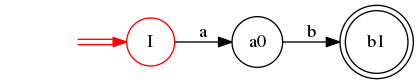
\includegraphics[width=0.5\linewidth]{figures/not_stretched.png}
\caption{Original automaton image. Code \ref{app:not_stretched_automaton}}
\label{fig:not_stretched_automaton}
\end{figure}

\begin{figure}[H]
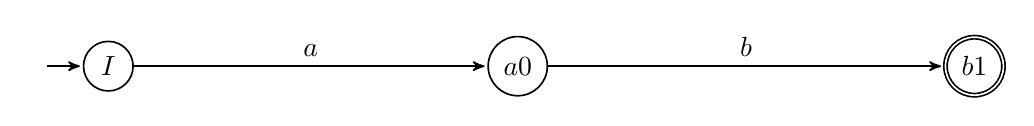
\begin{tikzpicture}[->,>=stealth',shorten >=1pt,auto,node distance=2.8cm,semithick,initial text=$ 	$]
	\tikzset{every state/.style={minimum size=0pt}}
	\node[state] (0) at (12.27,1.78) {$a0$};
	\node[state, accepting] (1) at (18.07,1.78) {$b1$};
	\node[state, initial, initial where=left] (2) at (7.07,1.78) {$I$};
	\path
		(0)

			edge  node {$b$} (1)
		(2)

			edge  node {$a$} (0);
\end{tikzpicture}
\caption{Example of a stretched automaton. Code \ref{app:stretched_automaton}}
\label{fig:stretched_automaton}
\end{figure}

This unwanted effect could be one of the areas to work on in the future (section \ref{sec:coordinate_upgrades}).

\subsection{Graphviz layout engines}
Graphviz has four main layout engines that can be used to draw automaton state diagrams:
\begin{itemize}
	\item dot
	\item neato
	\item circo
	\item twopi
\end{itemize}

There are also other engines: sfdp, fdp. These engines are not implemented in JASL, because sfdp and fdp are for undirected graphs.

These engines produce vastly different images. I got the best results using dot engine, but for some particular examples \textbf{circo} yields more visually appealing images.
 
\subsubsection{Example of layout difference}
We have an automaton $M$. This automaton has four states. These are the images of automaton $M$ generated by different layout engines:

\begin{figure}[H]
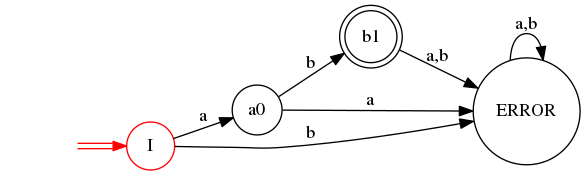
\includegraphics[width=0.8\linewidth]{figures/layouts_dot.png}
\caption{Image of automaton $M$ generated using \textbf{dot} layout}
\label{fig:layout_diff_dot}
\end{figure}

\begin{figure}[H]
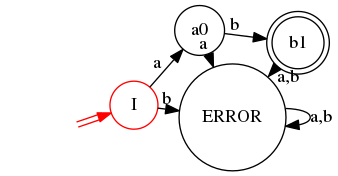
\includegraphics[width=0.7\linewidth]{figures/layouts_neato.png}
\caption{Image of automaton $M$ generated using \textbf{neato} layout}
\label{fig:layout_diff_neato}
\end{figure}

\begin{figure}[H]
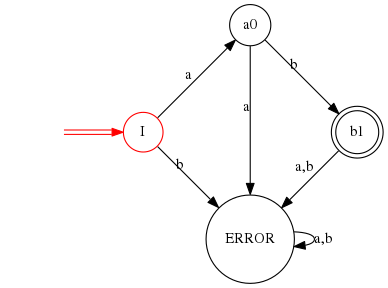
\includegraphics[width=0.7\linewidth]{figures/layouts_circo.png}
\caption{Image of automaton $M$ generated using \textbf{circo} layout}
\label{fig:layout_diff_circo}
\end{figure}

\begin{figure}[H]
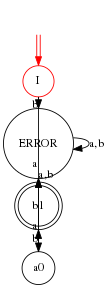
\includegraphics[width=0.2\linewidth]{figures/layouts_twopi.png}
\caption{Image of automaton $M$ generated using \textbf{twopi} layout}
\label{fig:layout_diff_twopi}
\end{figure}

Graphviz has an interesting feature. It varies the size of nodes according to the number of incoming/outgoing edges. This effect is apparent on foregoing figures.

\section{Relative position model}
\label{sec:relpos}
Originally, I wanted JASL to output TikZ code that would be the most easy for the user to edit. TikZ automata library was built to use the \textbf{relative} position model. In this model, every element of the graph is placed in relation to some other element. This allows for very easy editing of the image. For example, nodes of the graph on figure~\ref{fig:layout_diff_circo} could be described as follows:

\begin{verbatim}
	\node[state, initial] 	(0) 					{I};
	\node[state] 			(1) [above right of=0] 	{a0};
	\node[state] 			(2) [below right of=0] 	{ERROR};
	\node[state, accepting] (3) [below right of=1] 	{b1};
\end{verbatim}

This code can be quickly read and edited as opposed to absolute coordinates. TikZ allows nodes to be in eight different directions: above, above right, right, below right, below, below left, left, above left. Distance between nodes can be specified, but that clutters the code. TikZ places nodes on outer edge of a circle with diameter equal to the distance between nodes. One of the consequences of this feature is that sequence (below right, above right) does not give the same position as (right, right). There are only three types of edge shapes: bend left, bend right and straight. 

Using simplifications of the relative position TikZ code poses several constraints on the layout generator. Graphviz does not have support for these types of constraints. Graphviz has no attribute for ideal edge length or grid alignment of nodes. So the only option is to calculate/approximate these positions. However, this approximation destroys the layout completely at times. 

\subsection{Relation chains}
The relative model is easily editable, but only if the relations are connected correctly. The grouping of relations is a problem, because the program has to approximate, which nodes should be connected to which.

In this simple example, we have some graph, which is constructed using these relations:

\begin{enumerate}
	\item $1$ is to the right of $0$
	\item $4$ is to the right of $1$
	\item $5$ is under $4$
	\item $3$ is under $0$
	\item $2$ is to the right of $3$
\end{enumerate}

We can visualize these relations like this:

\begin{figure}[H]
\centering
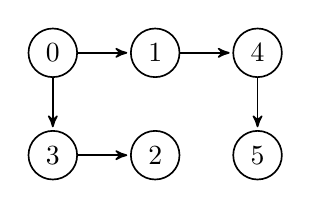
\begin{tikzpicture}[->,>=stealth',shorten >=1pt,auto,node distance=1.3cm,semithick,initial text=$ 	$]
	\tikzset{every state/.style={minimum size=0pt}}
	\node[state] (0) {$0$};
	\node[state] (1) [right of=0] {$1$};
	\node[state] (3) [below of=0] {$3$};
	\node[state] (2) [right of=3] {$2$};
	\node[state] (4) [right of=1] {$4$};
	\node[state] (5) [below of=4] {$5$};
	\path
		(0)

			edge  node {} (1)
			edge  node {} (3)
		(1)
			edge  node {} (4)
		(4)
			edge  node {} (5)
		(3)
			edge  node {} (2);
\end{tikzpicture}
\end{figure}

Suppose that we want to move nodes $1,4,5$ below node $2$. It is very easy, just by changing the relation of node $1$ to be: $1$ is below of $2$. The result will look like this:

\begin{figure}[H]
\centering
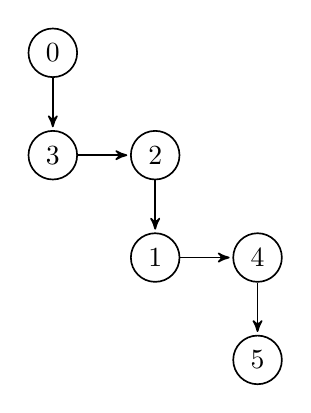
\begin{tikzpicture}[->,>=stealth',shorten >=1pt,auto,node distance=1.3cm,semithick,initial text=$ 	$]
	\tikzset{every state/.style={minimum size=0pt}}
	\node[state] (0) {$0$};
	\node[state] (3) [below of=0] {$3$};
	\node[state] (2) [right of=3] {$2$};
	\node[state] (1) [below of=2] {$1$};
	\node[state] (4) [right of=1] {$4$};
	\node[state] (5) [below of=4] {$5$};
	\path
		(0)
			edge  node {} (3)
		(2)
			edge  node {} (1)
		(1)
			edge  node {} (4)
		(4)
			edge  node {} (5)
		(3)
			edge  node {} (2);
\end{tikzpicture}
\end{figure}

Now suppose we have these relations in the graph:
\begin{figure}[H]
\centering
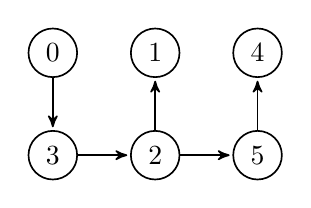
\begin{tikzpicture}[->,>=stealth',shorten >=1pt,auto,node distance=1.3cm,semithick,initial text=$ 	$]
	\tikzset{every state/.style={minimum size=0pt}}
	\node[state] (0) {$0$};
	\node[state] (3) [below of=0] {$3$};
	\node[state] (2) [right of=3] {$2$};
	\node[state] (1) [above of=2] {$1$};
	\node[state] (4) [right of=1] {$4$};
	\node[state] (5) [below of=4] {$5$};
	\path
		(0)
			edge  node {} (3)
		(2)
			edge  node {} (5)
			edge  node {} (1)
		(3)
			edge  node {} (2)
		(5)
			edge  node {} (4);
\end{tikzpicture}
\end{figure}

Now it is much more complicated to do this simple operation because to produce the wanted result, we have to change the relation of three nodes: $1, 4, 5$. 

Because we do not know, if and how the user wants to reorganize the output graph, there would have to be some utility, that would re-route the edges. Without this utility, the relation model would be of no use.

Because of these difficulties, I discarded the idea of relative positions and used absolute positions in the final version of the program.

\subsection{Edge angle calculation}
\label{subsec:edge-angle}
The Graphviz output dot file specifies edge shapes in the pos attribute. This attribute contains coordinates of several knot points, specifying a spline curve. As stated in previous section, there are three possible shapes of edges in TikZ automata library: straight, bend left, bend right. Approximation to those three edge shapes in TikZ produced mostly illegible images. 

The ultimate goal was to keep the TikZ code simple and easy to read. I decided to use the angles library for TikZ, that allows the user to specify the angle of the bend. The angle is a numeric value between $0^\circ$ and $360^\circ$, which specifies the angle $\alpha$ depicted in the following picture:

\begin{figure}[H]
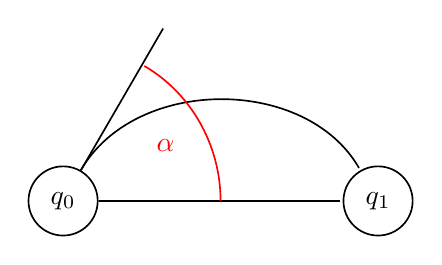
\begin{tikzpicture}[>=stealth',shorten >=1pt,auto,node distance=4cm,semithick,]
	\node[state] (0) at (0,0) {$q_0$};
	\node[state] (1) at (4,0) {$q_1$};
	\path (0) edge [bend left = 60] node{} (1);
	
	\draw (1.27,2.19) -- (0) -- (1);
	\draw[red] (2,0) arc (0:60:2cm);
	\draw[red] (1.3,0.7) node {$\alpha$};
  \end{tikzpicture}
\end{figure}

Bend left at $270^\circ$ produces the same output as bend right at $90^\circ$. I decided to keep TikZ code readable and unambiguous by using both directions (left and right), and limiting the angle to between $1^\circ$ to $179^\circ$.

I defined an function $f$ in the code of the application, that outputs this angle as well as the edge orientation. It takes three arguments: $\vec{q_0}, \vec{q_1}, P$, where $q_0$ is the source node center, $q_1$ is the destination node center and $P$ is a set of spline knot points. Function $f$ should return an angle. If the angle is negative, the curve is to the right, if it is positive, the curve is to the left, otherwise, it is to the right. 

Splines generated by Graphviz are generally simple, mostly elliptical. I used this property to approximate the curve angle using the following function::
\begin{align*}
	f(\vec{q_0}, \vec{q_1}, P) &= angle(\vec{q_1}, \vec{q_0}, \vec{p_*}) \cdot ((\vec{q_1} - \vec{q_0})\times sgn(\vec{p_*} - \vec{q_0})) \text{, where } \\
	\vec{p_*} &= \argmax_{\vec{p} \in P} (angle(\vec{q_1}, \vec{q_0}, \vec{p})) \\
	angle(\vec{a}, \vec{b}, \vec{c}) &= \frac{
		180 \cdot \arccos{ \vec{x} \cdot \vec{y} }}{ \pi \cdot |\vec{x}| \cdot |\vec{y}| }, \vec{x} = (\vec{a} - \vec{b}), \vec{y} = (\vec{c}-\vec{b})
\end{align*}

This function outputs angle $\gamma$ between $q_0, q_1$ and point $\vec{p_*} \in P$, which maximizes $\gamma$. 

While this function has good results when Graphviz uses elliptical edges, it is not so good otherwise. Graphviz uses elliptical splines only if the edges are short. If the edge exceeds certain length, it will flatten the spline curve. In these cases, angles output by function $f$ are not optimal. 

This function can be improved in the future (see \ref{par:angle-of-edges}).

\chapter{Examples of usage, practice, problems of testing}
Here are some examples of usage of the \textbf{JASL} language: 

\section{Defining a NFA automaton}
\label{sec:example_NFA}
Suppose we have regular language: 
\begin{equation*}
L_1 = \{w \mid w \text{ contains } aba \text{ as substring }\}, L_1 \subseteq \{a, b\}^*
\end{equation*} 
We design regular automaton $M$ such that $L(M) = L_1$. Example of such automaton could be this non-deterministic automaton:
\begin{table}[H]
\begin{ctucolortab}
\begin{tabular}{cc|cc}
\multicolumn{2}{c}{\bfseries $M_1$} & \bfseries $a$ & \bfseries $b$ \\\Midrule
$\rightarrow$ 	& $0$ & $0,1$ 	& $0$  \\
				& $1$ &  	& $2$  \\
				& $2$ & $3$		&  \\
$\leftarrow$	& $3$ & $3$		& $3$ 
\end{tabular}
\end{ctucolortab}
\caption{Transition table of automaton $M_1$.}
\label{fig:examples_NFA_table}
\end{table} 

In order to define automaton $M_1$ in JASL language we define a few lists: 

\begin{minipage}{\linewidth}
\begin{lstlisting}[language = JASL]
	|$alphabet| = {a, b}
	|$row0|  = {>, 0, {0,1}, 0}
	|$row1|  = {1, {}, 2}
	|$row2|  = {2, 3}
	|$row3|  = {<, 3, 3, 3}
    
	% Now we can define an automaton:
	|$M_1|  = Automaton({|$alphabet|, |$row0|, |$row1|, |$row2|, |$row3|})

	% We can get, whether automaton accepts word bbbbaab:
	|$accepted| = |$M_1|.accepts(bbbbaab)   
	% Accepted has value: false 
	
	% We can get regular expression describing the language L1:
	|$reg| = |$M_1|.toRegex()
	% $reg has value: b*aa*b((bb*aa*b)*)a((a+b)*) 

	% But does this regex really describe language L1? 
	% This one definitely does:
	|$regex| = (a+b)*aba(a+b)*
	|$M_2| = fromRegex($regex)
	|$M_2|.equals(|$M_1|) 	
	% Outputs: true
\end{lstlisting}
\end{minipage}

Note that we use nested lists for definitions of sets of target states. We can use $\{\}$ to denote $\emptyset$. The output of .getRegex() can be quite complicated. That is because no real regular expression simplifier has been implemented yet.

\section{Defining an ENFA automaton}
\label{sec:example_ENFA}
Suppose we have an ENFA automaton $M_2$ that accepts all words generated by regular expression: $a^* + b^*$.

Such automaton can be described by this transition table:
\begin{table}[H]
\begin{ctucolortab}
\begin{tabular}{cc|ccc}
\multicolumn{2}{c}{$M_2$} & $\varepsilon$ & $a$ & $b$ \\\Midrule
$\rightarrow$ 	& $S$ & $A,B$  \\
				& $A$ & $F$ 	& $A$  \\
				& $B$ & $F$		& & $B$ \\
$\leftarrow$	& $F$ & 		&  
\end{tabular}
\end{ctucolortab}
\caption{Transition table of automaton $M_2$.}
\label{fig:examples_DFA_table}
\end{table} 

We can define this automaton in JASL as follows:

\begin{minipage}{\linewidth}
\begin{lstlisting}[language = JASL]
	|$Sigma| = {eps, a, b}
	% We can even shorten the definition by the last empty transitions
	|$stateS| = {>, S, {A, B}}
	|$stateA| = {A, F, A}
	|$stateB| = {B, F, {}, B}
	|$stateF| = {<, F}
	|$M_2| = Automaton({|$Sigma|, |$stateS|, |$stateA|, |$stateB|, |$stateF|})
	
	% Now we can save png image of automaton M_2:
	|$M_2|.toPNG(image.png)	
\end{lstlisting}
\end{minipage}

The resulting image is:

\begin{figure}[H]
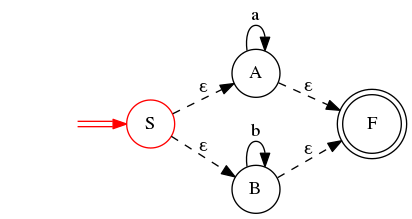
\includegraphics[width=0.8\linewidth]{figures/ENFA_definition.png}
\caption{Image saved in image.png}
\label{fig:ENFA_definition_example}
\end{figure}

\section{Example of TikZ image}
Suppose we have automaton $M_3$. This automaton accepts language $L = L(M_3)$. This language is also described by regular expression $\underline{r_2}$. 
\begin{equation*}
	\underline{r_2} = (a+b)^*ab^*, \hspace{1cm} L(M_3) = L_{\underline{r_2}} = L
\end{equation*}

We can use JASL to construct this automaton and create \TeX file to display it:

\begin{minipage}{\linewidth}
\begin{lstlisting}[language = JASL]
	|$a| = fromRegex((a+b)*ab*)
	% TeX document parts
	|$class| = \documentclass{article}
	|$includes| = getTikzIncludes()
	|$beginning| = \begin{document}
	|$tikzCode| = |$a|.toTikz()
	|$end| = \end{document}
	
	% Now append these parts in the image.tex file
	|$class|.save(image.tex)
	|$includes|.save(image.tex)
	|$beginning|.save(image.tex)
	|$tikzCode|.save(image.tex)
	|$end|.save(image.tex)
\end{lstlisting}
\end{minipage}

After compiling image.tex file we get this image:

\begin{figure}[H]
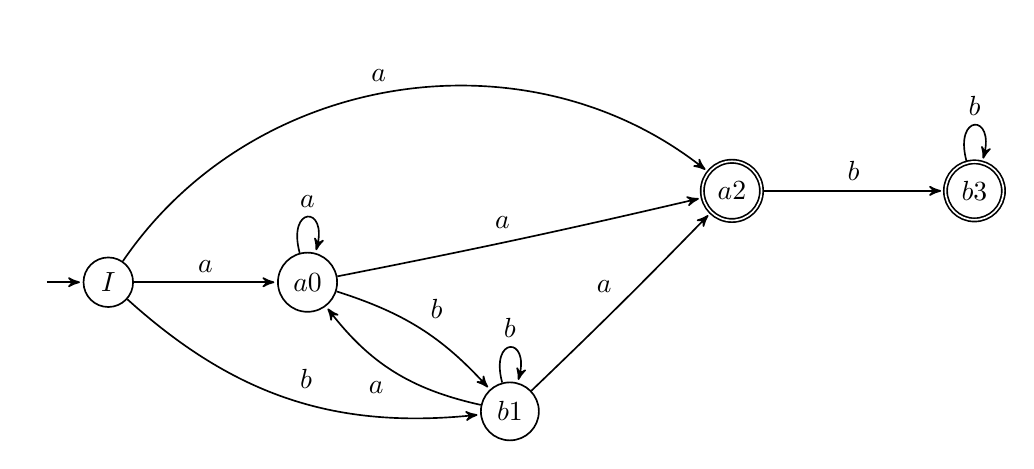
\begin{tikzpicture}[->,>=stealth',shorten >=1pt,auto,node distance=2.8cm,semithick,initial text=$ 	$]
	\tikzset{every state/.style={minimum size=0pt}}
	\node[state] (0) at (5.97,2.26) {$a0$};
	\node[state] (1) at (8.54,0.62) {$b1$};
	\node[state, accepting] (2) at (11.36,3.42) {$a2$};
	\node[state, accepting] (3) at (14.44,3.42) {$b3$};
	\node[state, initial, initial where=left] (4) at (3.44,2.26) {$I$};
	\path
		(0)

			edge [loop above] node {$a$} (0)
			edge [bend left = 15] node {$b$} (1)
			edge [bend right = 1] node {$a$} (2)
		(1)

			edge [bend left = 20] node {$a$} (0)
			edge [loop above] node {$b$} (1)
			edge [bend right = 1] node {$a$} (2)
		(2)

			edge  node {$b$} (3)
		(3)

			edge [loop above] node {$b$} (3)
		(4)

			edge  node {$a$} (0)
			edge [bend right = 24] node {$b$} (1)
			edge [bend left = 47] node {$a$} (2);
\end{tikzpicture}
\caption{Image in compiled image.pdf file.}
\label{fig:compilation_tikz_code}
\end{figure}

\section{Example of a JASL script file}
\label{ex:exec-overwrite}
In this example, we can see the execution of JASL script file and the side effects of using execute function.

Suppose we have a file append.jasl, that contains the code that will concatenate the language produced by regular expression: $ab^*a$ to language accepted by automaton saved in variable \textbf{\$i}. It will save the result to variable \textbf{\$j}. Such file could contain for example this code:

\begin{minipage}{\linewidth}
\begin{lstlisting}[language = JASL]
	|$append| = fromRegex(ab*a)
	|$j| = |$i|.concatenation(|$append|)
\end{lstlisting}
\end{minipage}

We can check whether the function worked correctly:

\begin{minipage}{\linewidth}
\begin{lstlisting}[language = JASL]
	|$i| = fromRegex(bba)
	% We define the append variable
	|$j| = hello
	|$shouldBe| = fromRegex((bba)(ab*a))

	execute(append.jasl)
	
	% We can see that the contents of the variable k were overwritten:
	|$j|.equals(|$shouldBe|)
\end{lstlisting}
\end{minipage} 

The last command will print true to console. Note that by executing code in append.jasl we have overwritten anything that might be in the variable \textbf{\$j}. The user has to be aware of this side effect. Stack frames might be implemented later~\ref{sec:interpreter_upgrades}

\chapter{Looking to the future}
\label{todo}

JASL and its interpreter do not yet implement some of the features that I would want them to. The ultimate goal of this application is to make tasks regarding automata simple. There are many quality-of-life improvements that yet wait to be implemented. I will describe some of those features in this chapter.

\section{JAutomata}
The JAutomata library could implement other types of automata (Mealy, Moore, Push-down) because these types of automata are often used in practice. The implementation could use the structure of the project and its classes with minor tweaks. 

\subsection{Operations over regular expressions}
The regular expression format used in JAutomata library, which is also defined in this thesis differs from the format that is usually used in literature. It does not implement powers of regular expressions and positive iteration operator. 
\subsubsection{Power of regular expression}
Powers of regular expressions are often used to shorten regular expressions with repeating symbols.

\paragraph{Definition of power of regular expression}
Suppose we have regular expression $\mathbf{r}$ that describes language $L$. Then regular expression $\mathbf{r^i}$ describes language $L^i$ which can be defined recursively as:
\begin{itemize}
	\item $L^0 = \{\varepsilon\}$
	\item $L^{n+1} = LL^{n}$
\end{itemize} 

\subsubsection{Positive iteration}
Another operator missing from the implementation is the positive iteration of regular expressions.

\paragraph{Definition of positive iteration} Suppose we have a language $L$ that is described by regular expression $\mathbf{r}$. Then regular expression $\mathbf{r^+}$ describes language $L^+$ which is the positive iteration of the language $L$ and can be defined as:
\begin{equation*}
L^+ = \bigcup_{i=1}^\infty L^i
\end{equation*}

Both of these operators are only shortened versions of regular expressions. For example, regular expression $\mathbf{r^+}$ can be denoted by $\mathbf{rr^*}$, without changing the resulting language.

\subsection{Regular expression simplifier}
For the moment, the library is missing any regular expression simplifier. Problem of regular expression minimization is computationally hard (PSPACE-complete as shown in~\cite{np-regex}). This could be implemented using already existing algorithms that yield "good enough" results~\cite{simplifying-regex}. 

\section{JASL}
JASL could implement additional features to make the enhance the user experience. In this section I will focus on those improvements. 

\subsection{JASL Syntax}
JASL syntax could use some more advanced features. Such as: element extraction from a list or a string, user-defined functions, other data-types or allowing the user to use some of the more advanced features of JAutomata library. It could also make possible the modification of generated PNG images (colors of edges, size of the image, etc.). These changes would make JASL more flexible for the user.

Standardization of the syntax would help users that are used to working with regular programming languages. One example of such standardization would be encapsulation of strings in double quotes. This would allow for better exception handling and syntax error detection.

\subsection{Interpreter}
\label{sec:interpreter_upgrades}
Examples of possible upgrades to the JASL interpreter are:
\begin{itemize}
	\item Making error messages more clear
	\item Implementing command that would print all used variables
	\item Implementing stack frames for script executions
	\item Saving current workspace (state of all variables) to a file
	\item Live preview of generated images
	\item Live console code completion
\end{itemize}

Apart from stak frames, all of these upgrades are a quality-of-life improvements. For example the live preview of generated images would certainly enhance the user experience. Live code completion for the live console environment would probably require to implement custom console. 

\subsection{Graph conversion}
\label{sec:coordinate_upgrades}
The JASL language could implement the relative position model, as described in section~\ref{sec:relpos}. The problem is complicated to fine-tune and it would be necessary to implement some tool to change relations in the graph. If this feature is implemented, adding live preview of graphs would be advisable.

\paragraph{Coordinate conversion}
As described in section~\ref{sec:problems_graphviz}, the current implementation of dot to Tikz coordinate conversion stretches small graphs. One way of dealing with this stretching is to calculate the required distance between nodes. The calculation would compare the size of the node from the dot code to the distance between nodes. Based on the result it would decide, how distant the nodes should be. There are lots of constants in such calculation, that would require fine-tuning and a lot of experimnetation.

\paragraph{Angle of edges}
\label{par:angle-of-edges}
Upgrade of the function $f$, described in section \ref{subsec:edge-angle} would improve diagrams of automata with longer edges. This function should be implemented to \textbf{cz.cvut.fel.horovtom.jasl.graphviz.DotToTex.getCurveAngle} function. Graphviz does not curve longer edges evenly. Such an edge can be seen on the following picture from state 0 to state 4.

\begin{figure}[H]
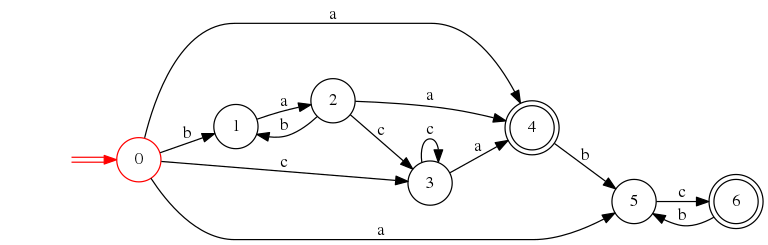
\includegraphics[width=1\linewidth]{figures/not-round-edge.png}
\caption{Image of longer edge}
\label{fig:longer-edge}
\end{figure}

When converting this automaton to TikZ, we can see, that the current function does a decent job:

\begin{figure}[H]
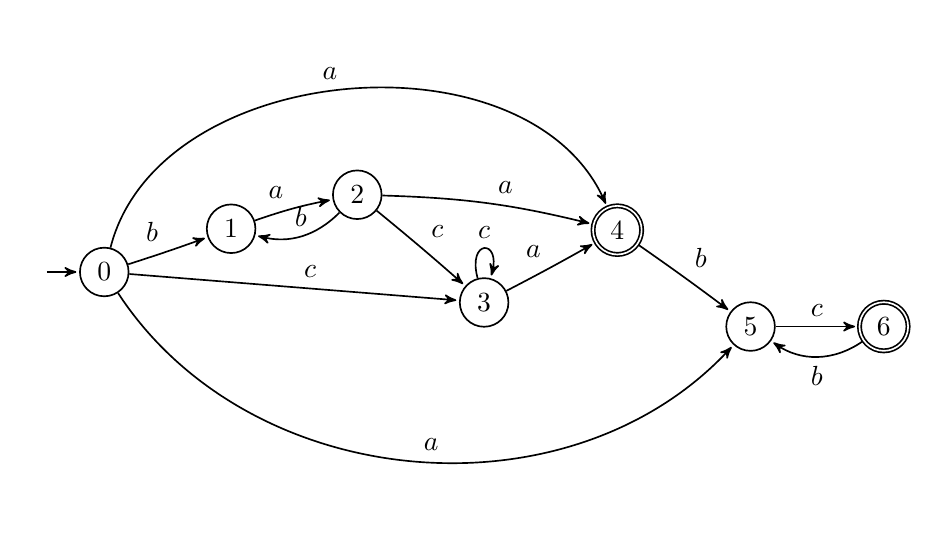
\begin{tikzpicture}[->,>=stealth',shorten >=1pt,auto,node distance=2.8cm,semithick,initial text=$ 	$, scale=0.9]
	\tikzset{every state/.style={minimum size=0pt}}
	\node[state, initial, initial where=left] (0) at (2.47,1.47) {$0$};
	\node[state] (1) at (4.26,2.08) {$1$};
	\node[state] (2) at (6.04,2.56) {$2$};
	\node[state] (3) at (7.83,1.04) {$3$};
	\node[state, accepting] (4) at (9.71,2.06) {$4$};
	\node[state] (5) at (11.59,0.70) {$5$};
	\node[state, accepting] (6) at (13.47,0.70) {$6$};
	\path
		(0)

			edge [bend right = 1] node {$b$} (1)
			edge  node {$c$} (3)
			edge [bend left = 71] node {$a$} (4)
			edge [bend right = 52] node {$a$} (5)
		(1)

			edge [bend left = 4] node {$a$} (2)
		(2)

			edge [bend left = 30] node  [above]{$b$} (1)
			edge [bend left = 1] node {$c$} (3)
			edge [bend left = 6] node {$a$} (4)
		(3)

			edge [loop above] node {$c$} (3)
			edge [bend right = 1] node {$a$} (4)
		(4)

			edge [bend left = 1] node {$b$} (5)
		(5)

			edge  node {$c$} (6)
		(6)

			edge [bend left = 35] node {$b$} (5);
\end{tikzpicture}
\end{figure}

However, on some pictures, the curvature is necessary to maintain clarity in the layout. In these cases TikZ can visualize edges of this shape much better with edge angle greater than $90^\circ$:
\begin{figure}[H]
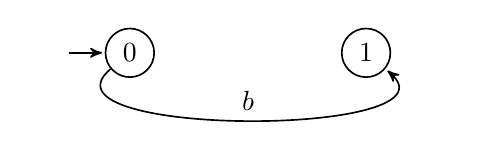
\begin{tikzpicture}[->,>=stealth',shorten >=1pt,auto,node distance=2.8cm,semithick,initial text=$ 	$]
	\tikzset{every state/.style={minimum size=0pt}}
	\node[state, initial, initial where=left] (0) at (0,0) {$0$};
	\node[state] (1) at (3,0) {$1$};
	\path
		(0)

			edge [bend right = 140] node {$b$} (1);
\end{tikzpicture}
\end{figure}

This could one of the possible improvements of the function $f$. 

\chapter{Conclusion}
The goals of this project were:
\begin{itemize}
	\item To finish implementation of regular expressions in JAutomata library
	\item To create a language, that could be used to define/work with regular automata
	\item To implement a live-console interpreter for this language
	\item To implement a mechanism for creation of dot code for drawing state diagrams of regular automata
	\item To implement a mechanism for conversion of attributed dot code to TikZ code.
\end{itemize}

All of these goals have been reached. Some areas might be improved in the future (see chapter \ref{todo}), but the application fulfills all set goals at the moment. Newer versions of the application code are accessible in the project github repository \cite{repo}. 

On the appended CD there is the project root directory and the pom.xml file, which allows for easy compilation of the project (as described in section \ref{compile}) and a pre-compiled .jar file of the project. 


\begin{thebibliography}{1}
	\bibitem{demlova} Marie Demlova. \emph{Jazyky, automaty a gramatiky.} Materials for CTU course Jazyky, Automaty a Gramatiky, 2017. \url{http://math.feld.cvut.cz/demlova/teaching/jag/jag7dohromady.pdf} 
	\bibitem{hopcroft} John E. Hopcroft, Jeffrey D. Ullman. \emph{Formal Languages and Their Relation to Automata}. Addison-Wesley Pub. Co., 1969. 
	\bibitem{graphviz} Graphviz official website. \url{https://www.graphviz.org/}.
	\bibitem{graphviz-java} Graphviz-java official repository. \url{https://github.com/nidi3/graphviz-java}
	\bibitem{tikz-tut} Satyaki Sikdar. \emph{Drawing Finite State Machines in \LaTeX using TikZ A Tutorial.} University of Notre Dame, 2017. \url{https://www3.nd.edu/~kogge/courses/cse30151-fa17/Public/other/tikz_tutorial.pdf}
	
	\bibitem{alg_lib_toolkit} Jan Travnicek and col. Private Gitlab repository of Algorithms Library Toolkit developed at FIT CVUT, accessible with CVUT credentials. \url{https://gitlab.fit.cvut.cz/algorithms-library-toolkit/automata-library}
	\bibitem{melichar} Bořivoj Melichar. \emph{Jazyky a Překlady.} CVUT, 2003.	
	
	\bibitem{acceptor-algorithm} Borivoj Melichar, Jan Holub, Tomas Polcar. \emph{Text searching algorithms.} CTU Prague, 2005. Algorithm p.203. \url{http://www.stringology.org/athens/TextSearchingAlgorithms/tsa-lectures-1.pdf#page=203}
	
	\bibitem{dot-notation} Manual for DOT language \url{https://www.graphviz.org/doc/info/lang.html}
	
	\bibitem{tikz-notation} Manual for TikZ automata library \url{https://www.bu.edu/math/files/2013/08/tikzpgfmanual.pdf} p.175-180
	
	\bibitem{tex} \TeX Users Group website. \url{http://tug.org/}
	
	\bibitem{repo} The official repository for JAutomata library and JASL projects \url{https://github.com/Horovtom/jAutomata}

	\bibitem{maven} The official website of Apache Maven \url{https://maven.apache.org/}	
	
	\bibitem{jdk} JDK8 download page \url{https://www.oracle.com/technetwork/java/javase/downloads/jdk8-downloads-2133151.html}
	
	\bibitem{school-notes} Tomas Horovsky. Notes for the A4B01JAG CVUT course \url{https://github.com/Horovtom/SchoolNotes/blob/master/A4B01JAG/A4B01JAG.pdf}
	
	\bibitem{simplifying-regex} H. Gruber, S. Gulan. \emph{Simplifying Regular Expressions
A Quantitative Perspective}. Universitat Gießen, 2009. \url{https://www.researchgate.net/profile/Hermann_Gruber3/publication/228529267_Simplifying_Regular_Expressions_A_Quantitative_Perspective/links/02e7e517274e7a8f6e000000/Simplifying-Regular-Expressions-A-Quantitative-Perspective.pdf}
	
	\bibitem{crossing-problem} Michael R. Garey,  David Johnson. \emph{Crossing Number is NP-Complete}. SIAM Journal on Algebraic and Discrete Methods. 4. 312-316. 10.1137/0604033, 1983.
	\bibitem{np-regex}  A.R. Meyer, L.J. Stockmeyer, The equivalence problem for regular expressions with squaring requires exponential space, in: Proc. 13th Ann.
IEEE Symp. on Switching and Automata Theory, 1972, pp. 125–129
\end{thebibliography}

\appendix
\chapter{Used code}
\section{Used DOT code}
This appendix includes all dot codes used to draw images.

\subsection{\ref{fig:not_stretched_automaton}}
\label{app:not_stretched_automaton}
\begin{minipage}{\linewidth}
\begin{lstlisting}
digraph automaton {
	graph [bb="0,0,306,55", rankdir=LR, size="8,3"];
	node [color=black, label="\N", shape=circle];
	qS0	 [color="", height=0.5, label="", pos="27,27.5", 
		shape=none, width=0.75];
	I	 [color=red, height=0.5, pos="109,27.5",
		width=0.5];
	qS0 -> I	 [color="red:invis:red",
		pos="e,90.826,27.5 54.195,27.5 62.654,27.5 72.051,27.5 80.595,27.5"];
	a0	 [height=0.52778, pos="189,27.5", width=0.52778];
	I -> a0	 [label=a,
		lp="148.5,35",
		pos="e,169.92,27.5 127.31,27.5 136.8,27.5 148.81,27.5 159.63,27.5"];
	b1	 [color="", height=0.76389,
		pos="278.5,27.5",
		shape=doublecircle,
		width=0.76389];
	a0 -> b1	 [label=b, lp="229.5,35",
		pos="e,250.75,27.5 208.13,27.5 217.56,27.5 229.44,27.5 240.69,27.5"];
}
\end{lstlisting}
\end{minipage}

\section{Used TikZ code}

\subsection{\ref{fig:stretched_automaton}}
\label{app:stretched_automaton}

\begin{minipage}{\linewidth}
\begin{lstlisting}
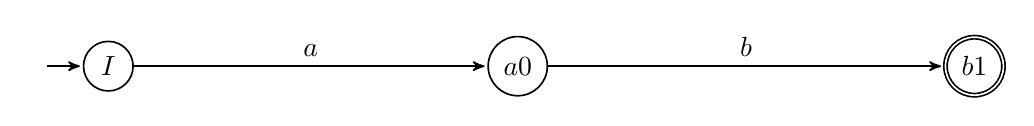
\begin{tikzpicture}[->,>=stealth',shorten >=1pt,auto,node distance=2.8cm,semithick,initial text=$ 	$]
	\tikzset{every state/.style={minimum size=0pt}}
	\node[state] (0) at (12.27,1.78) {$a0$};
	\node[state, accepting] (1) at (18.07,1.78) {$b1$};
	\node[state, initial, initial where=left] (2) at (7.07,1.78) {$I$};
	\path
		(0)

			edge  node {$b$} (1)
		(2)

			edge  node {$a$} (0);
\end{tikzpicture}
\end{lstlisting}
\end{minipage}

%TODO ADD FOR UPLOAD
%\ctutemplate{specification.as.chapter}

\end{document}

%\begin{figure}
%\includegraphics[width=0.8\linewidth]{mygraphicfile.pdf}
%\caption{We depict a foo-bar here.}
%\label{fig:foobar}
%\end{figure}

%\begin{table}
%\begin{ctucolortab}
%\begin{tabular}{cc}
%\bfseries Foo & \bfseries Bar \\\Midrule
%foo1 & bar1 \\
%foo2 & bar2
%\end{tabular}
%\end{ctucolortab}
%\caption{Table of foo-bar.}
%\label{tab:foobar}
%\end{table}
